254. При удалении крайних клеток периметр полоски не поменяется, а при удалении соседних поменяется в сумме на 2, а должен на $48-(20+2)\cdot2=4.$ Значит, клетки необходимо удалять не крайние, не соседние и не приводящие к разваливанию полоски. Последовательно заполним полоску, написав в каждой клетке количество способов выбрать для неё вторую удаляемую клетку.
\begin{center}
\begin{figure}[ht!]
\center{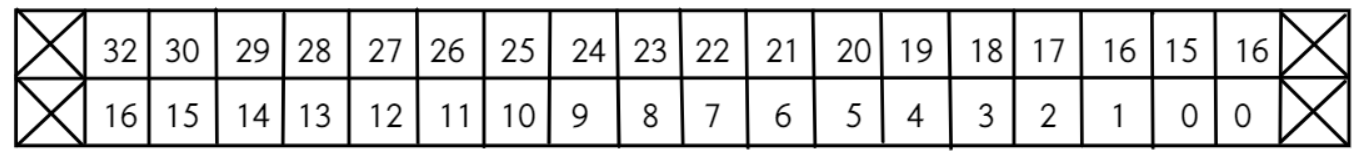
\includegraphics[scale=0.3]{gg.png}}
\end{figure}
\end{center}
Так как крайние клетки брать нельзя, изначально для выбора остаётся $2\cdot20-4=36$ клеток. Вместе с левой верхней клеткой нельзя брать её саму и 3 её соседей, остаётся $36-4=32$ возможных клетки. Вместе со второй клеткой в верхнем ряду нельзя брать её саму и 5 соседей, остаётся $36-6=30$ возможных клеток. Далее у каждой следующей клетки будет на 1 вариант меньше (нельзя брать ранее рассмотренные клетки), пока мы не дойдём до последней клетки. Двумя её соседями являются изначально запрещённые крайние клетки, поэтому с ней можно брать $15-1+2=16$ клеток. Вместе с крайней левой клеткой нижней строки можно взять все клетки нижней строки кроме трёх с левого края и одной с правого, то есть опять $20-4=16$ клеток. Далее количество вариантов опять уменьшаться на 1, пока не дойдёт до 0. Значит, всего вариантов будет $32+30+29+28+\ldots+16+15+16+16+15+14+\ldots+2+1=1+2+\ldots+29+30+16+15+16+32=(1+30)+(2+29)+\ldots+(15+16)+79=31\cdot15+79=544.$\newpage\noindent
